\chapter{Opis projektnog zadatka}
		
Cilj ovog projekta je razviti aplikaciju za učenje stranog jezika koja se bazira na ponavljanju s odmakom (još i poznato pod „spaced repetition“). Popularne aplikacije kao što su Quizlet, Anki te Memrise. Nove riječi se uče postavljanjem pitanja o riječima koje su prethodno definirane u bazi riječi. Učenik odgovara s prijevodima riječi odabirući ispravan odabir od nekoliko ponuđenih alternativnih riječi. Ako učenik točno odgovori na pitanje, riječ koja se nalazi u pitanju se pomiče u sljedeću skupinu/posudu riječi, no ako učenik netočno odgovori na pitanje, riječ će se vratiti na „početak“ odnosno u prvu skupinu/posudu riječi koje se smatraju ne naučenima. Svaka skupina, koje su međusobno povezane u niz, ima određeno vrijeme „trajanja“ prema čijem isteku riječ postaje ponovno dostupna za prikazivanje učeniku u formi pitanja. Vrijeme trajanja za prvu skupinu koja se nalazi u nizu je jedan dan, druga skupina u nizu ima vrijeme trajanja od 2 dana te se za svaku sljedeću skupinu broj dana udvostručuje. Aplikacija ima        broj posuda te ako se riječ nalazi u posljednjoj od povezanih posuda, tada se po isteku vremena riječ smatra naučenom te se smješta u posebnu posudu i više ne sudjeluje u učenju strane riječi. 

Administrator dodaje strane riječi, iz odabranog stranog jezika, u aplikaciju. Uzmimo za primjer engleski jezik kako bi pokazali funkcionalnost aplikacije. Svaka riječ koja će se učiti se sastoji od engleske riječi, opisa riječi koji je sačinjen od nekoliko fraza ili rečenica, prijevoda engleske riječi na hrvatski te nekoliko rečenica/fraza koje je bolje opisuju te na posljetku glasovne datoteke izgovora na engleskom jeziku. Svaka riječ koja je dodana u bazu se može obrisati ili joj se mogu promijeniti komponente. Riječi su povezane u rječnike koji se sastoje od imena i riječi. Nove riječi se mogu dodati u jedan ili više otprije postojanih rječnika. Kod definiranja riječi, administrator riječi ima pomoć u obliku savjeta koji su prikupljeni od strane vanjskog izbora. Aplikacija komunicira s vanjskim rječnikom (https://rapidapi.com/collection/thesaurus-apis) kada administrator upiše dio riječi te pokrene proceduru pretrage preko koje se prihvaćaju riječi i njezini opisi. 

Učenik/korisnik se može registrirati putem elektroničke pošte i promijeniti lozinku. Prilikom prvog login-a se na korisnikovu elektroničku poštu šalje privremena lozinka koja se mora promijeniti. 
Atributi korisničkog/učeničkog računa: 
\item[1]. Elektronička pošta 
\item[2]. Lozinka 
Učenik odabire jedan od ponuđenih rječnika te može pokrenuti učenje riječi. 
Učenje riječi se može odvijati kroz nekoliko različitih mode-ova
Mode-ovi:
\item[1].	Upit engleske riječi uz odabir hrvatskog prijevoda 
\item[2].	Upit hrvatske riječi uz odabir engleskog prijevoda
\item[3].	Upit izgovorom engleske riječi uz pisanje riječi na engleskom (provjera ispravnog pisanja)
\item[4].	Upit tekstualnim oblikom engleske riječi uz snimanje izgovora u zvučnu datoteku
Netočni odgovori ponuđeni studentu se izabiru slučajnim odabirom iz skupine odgovora koji moraju biti istog tipa drugih rječnika kod mode-ova učenja gdje se prezentira više opcija odabira. Za kontrolu snimljenih datoteka u kojima su izgovorene riječi stranog jezika „postoji“ servis koji kontrolira točnost izgovorenih riječi i vraća povratnu ocjenu. Implementirano je i umjetno aplikacijsko sučelje koje će prihvatiti takvu glasovnu datoteku te će povratno vratiti ocjenu na ljestvici od 1 do 10. 

Bez obzira koji jezik učili, funkcionalnosti su jednako implementirane za sve jezike. Svaki rječnik ima dodatnu oznaku kako bi se znalo na koji jezik se on odnosi te sadrži riječi samo jednog jezika. Rječnici su grupirani po jeziku te se takvi prikazuju učeniku/korisniku prilikom odabira rječnika. 

Hijerarhijski postoji glavni administrator sa najvećim ovlastima koje su mu korijenski dodijeljene. On može druge korisničke/učeničke račune „unaprijediti“ u administratore koji će imati jednake ovlasti kao i on sam. Učenički računi ne ovise o administratorskim te se oni sami registriraju i brišu svoj korisnički račun po potrebi.

Za kraj opisa projekta proći ćemo kroz aplikaciju po imenu Quizlet, ranije navedenu, te ćemo pogledati njihov način implementacije.

\begin{figure}[H]
	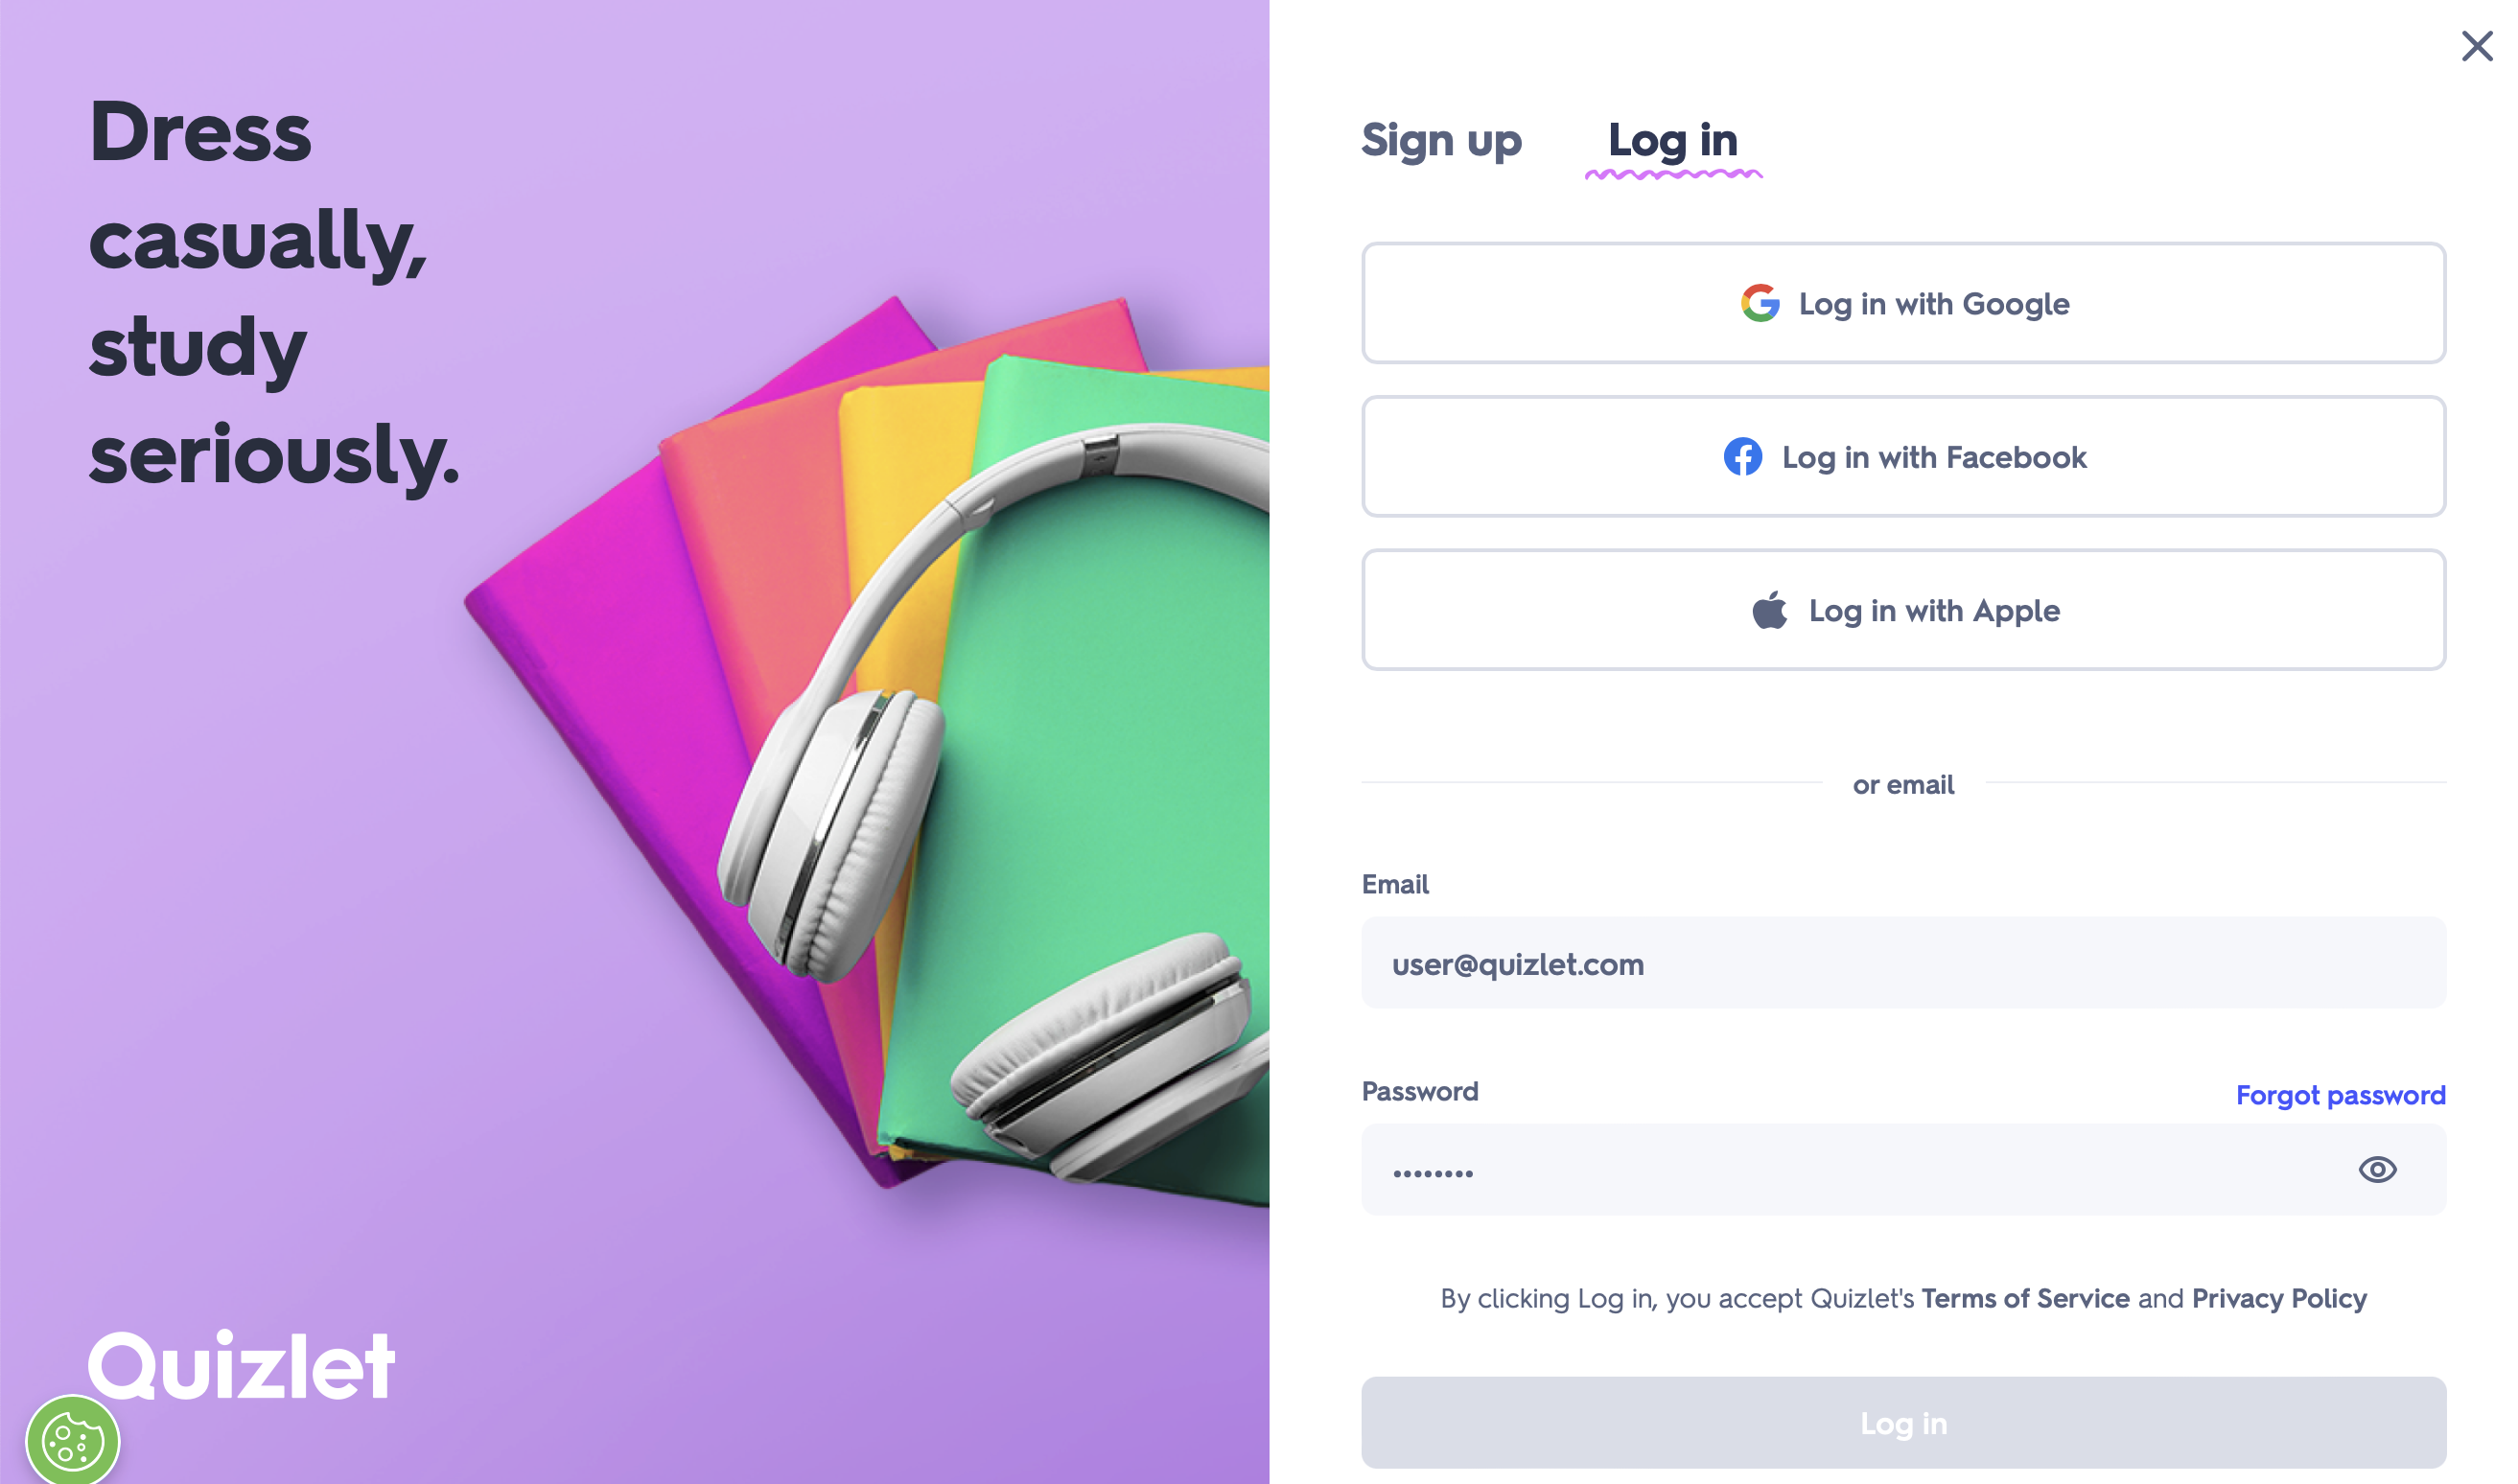
\includegraphics[width=\textwidth]{SlikeOpisProjekta/login_screen_quizlet.png} %veličina u odnosu na širinu linije
	\caption{Slika login stranice Quizeta}
	\label{fig:LoginScreenQuizlet} %label mora biti drugaciji za svaku sliku
\end{figure}

Prilikom ulaska na stranicu možemo birati između dva oblika prijave:
\item[1]. Log in
\item[2]. Sign up

U slučaju da već imamo korisničku račun odabrat ćemo opciju Log in, a inače Sign up. Također postoje i opcije login-a sa Apple, Google ili Facebook računom. 

\begin{figure}[H]
	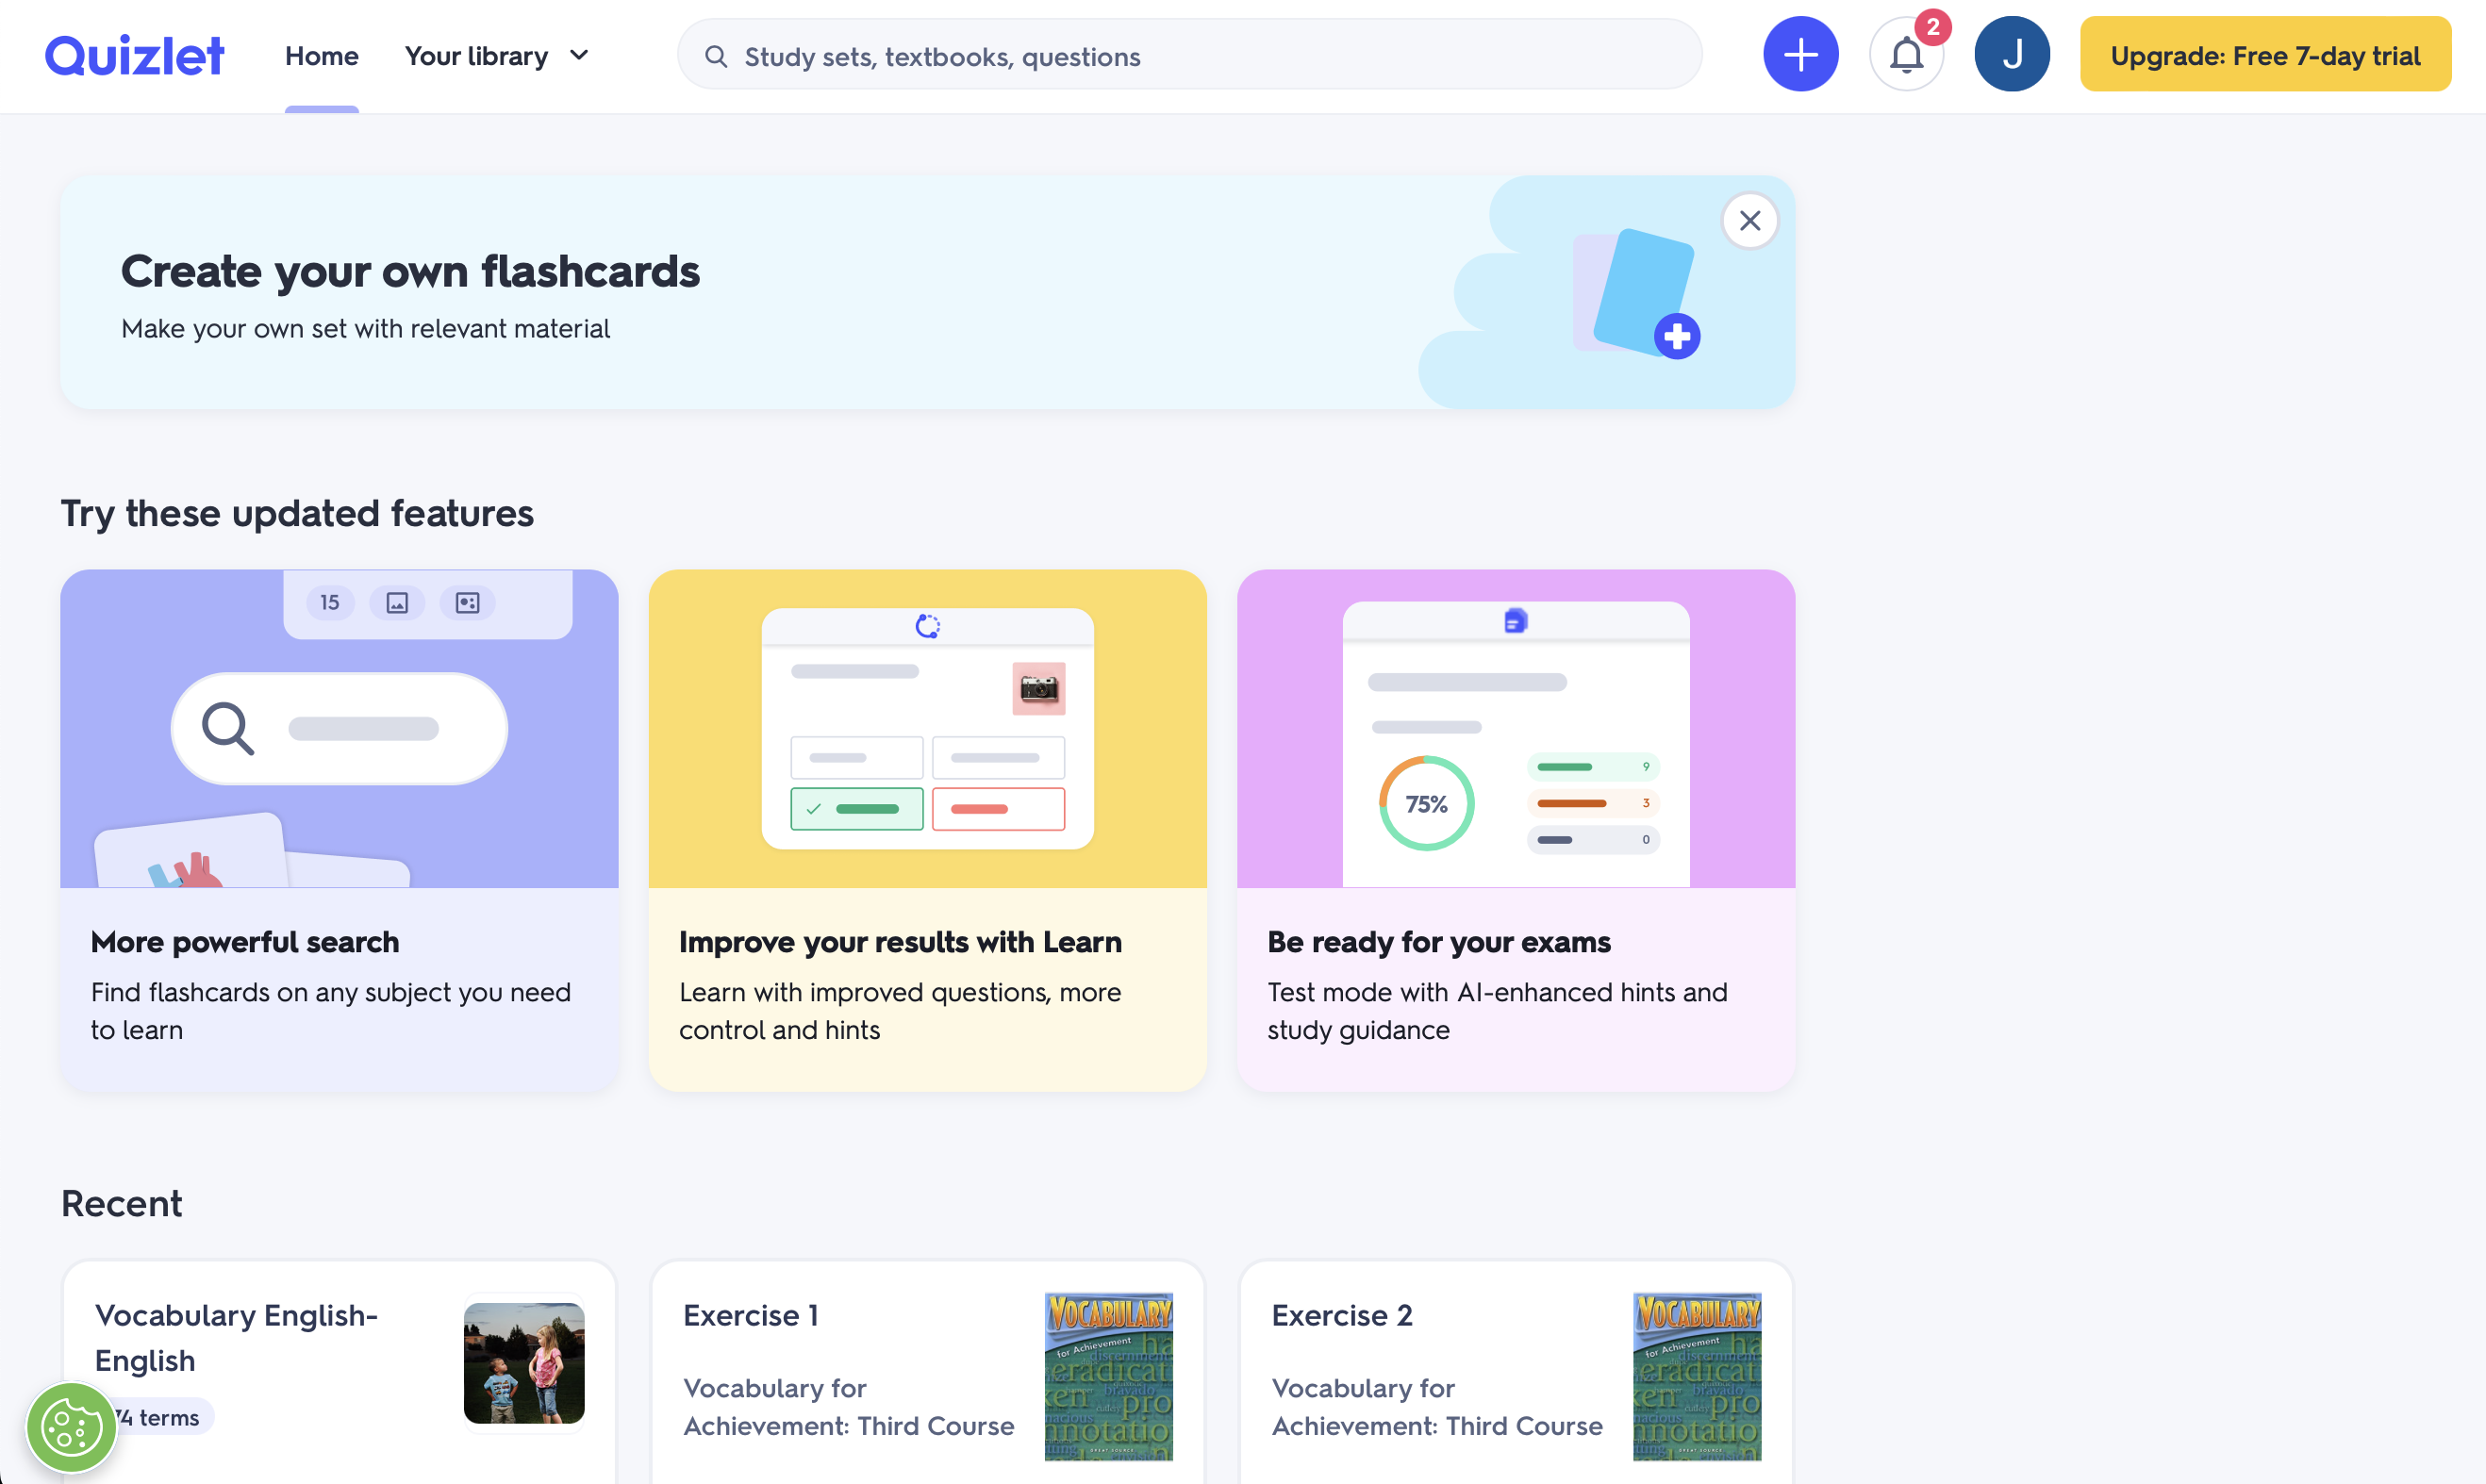
\includegraphics[width=\textwidth]{SlikeOpisProjekta/user_interface_quizlet.png} %veličina u odnosu na širinu linije
	\caption{Slika ui stranice}
	\label{fig:UserInterfaceQuizlet} %label mora biti drugaciji za svaku sliku
\end{figure}

Poslije login-a u svoj stari/novokreirani korisnički račun dolazimo do sučelja gdje korisnik bira što i na koji način želi učiti. Iskoristit ćemo već napravljeni kviz za učenje engleskog jezika te ćemo na njemu demonstrirati mogućnosti aplikacije. 

\begin{figure}[H]
	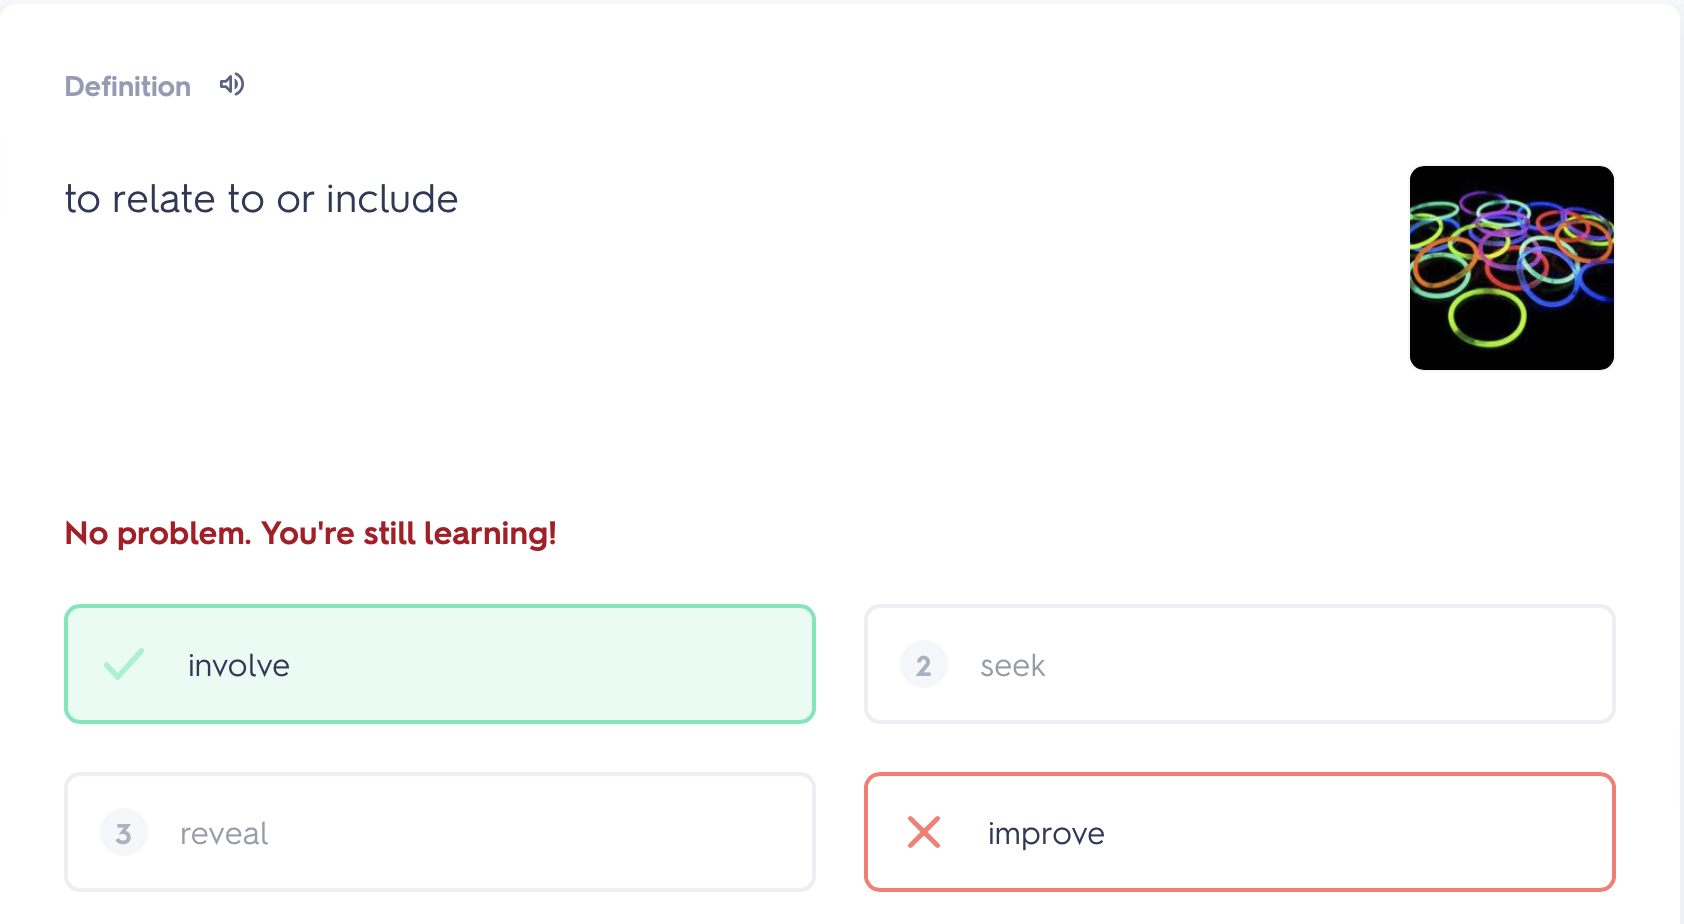
\includegraphics[width=\textwidth]{SlikeOpisProjekta/english_quiz_wrong_answer_quizlet.png} %veličina u odnosu na širinu linije
	\caption{Kviz krivi odgovor}
	\label{fig:EnglishQuizWrongAnswerQuizlet} %label mora biti drugaciji za svaku sliku
\end{figure}

Na slici imamo prikazan kratki opis tražene riječi te imamo ponuđena 4 odgovora od kojih je samo jedan točan. Postoji i mogućnost čitanja teksta za osobe sa posebnim potrebama.
U slučaju krivog odgovora aplikacija pauzira daljnje učenje te nam ukazuje na pogrešku i daje malu motivacijsku poruku kako i dalje učimo, a u slučaju točnog odgovora nas pohvali te nastavi sa daljnjim pitanjima.

		\eject
		
		\section{Primjeri u \LaTeX u}
		
		\textit{Ovo potpoglavlje izbrisati.}\\

		U nastavku se nalaze različiti primjeri kako koristiti osnovne funkcionalnosti \LaTeX a koje su potrebne za izradu dokumentacije. Za dodatnu pomoć obratiti se asistentu na projektu ili potražiti upute na sljedećim web sjedištima:
		\begin{itemize}
			\item Upute za izradu diplomskog rada u \LaTeX u - \url{https://www.fer.unizg.hr/_download/repository/LaTeX-upute.pdf}
			\item \LaTeX\ projekt - \url{https://www.latex-project.org/help/}
			\item StackExchange za Tex - \url{https://tex.stackexchange.com/}\\
		
		\end{itemize} 	


		
		\noindent \underbar{podcrtani tekst}, \textbf{podebljani tekst}, 	\textit{nagnuti tekst}\\
		\noindent \normalsize primjer \large primjer \Large primjer \LARGE {primjer} \huge {primjer} \Huge primjer \normalsize
				
		\begin{packed_item}
			
			\item  primjer
			\item  primjer
			\item  primjer
			\item[] \begin{packed_enum}
				\item primjer
				\item[] \begin{packed_enum}
					\item[1.a] primjer
					\item[b] primjer
				\end{packed_enum}
				\item primjer
			\end{packed_enum}
			
		\end{packed_item}
		
		\noindent primjer url-a: \url{https://www.fer.unizg.hr/predmet/proinz/projekt}
		
		\noindent posebni znakovi: \# \$ \% \& \{ \} \_ 
		$|$ $<$ $>$ 
		\^{} 
		\~{} 
		$\backslash$ 
		
		
		\begin{longtblr}[
			label=none,
			entry=none
			]{
				width = \textwidth,
				colspec={|X[8,l]|X[8, l]|X[16, l]|}, 
				rowhead = 1,
			} %definicija širine tablice, širine stupaca, poravnanje i broja redaka naslova tablice
			\hline \SetCell[c=3]{c}{\textbf{naslov unutar tablice}}	 \\ \hline[3pt]
			\SetCell{LightGreen}IDKorisnik & INT	&  	Lorem ipsum dolor sit amet, consectetur adipiscing elit, sed do eiusmod  	\\ \hline
			korisnickoIme	& VARCHAR &   	\\ \hline 
			email & VARCHAR &   \\ \hline 
			ime & VARCHAR	&  		\\ \hline 
			\SetCell{LightBlue} primjer	& VARCHAR &   	\\ \hline 
		\end{longtblr}
		

		\begin{longtblr}[
				caption = {Naslov s referencom izvan tablice},
				entry = {Short Caption},
			]{
				width = \textwidth, 
				colspec = {|X[8,l]|X[8,l]|X[16,l]|}, 
				rowhead = 1,
			}
			\hline
			\SetCell{LightGreen}IDKorisnik & INT	&  	Lorem ipsum dolor sit amet, consectetur adipiscing elit, sed do eiusmod  	\\ \hline
			korisnickoIme	& VARCHAR &   	\\ \hline 
			email & VARCHAR &   \\ \hline 
			ime & VARCHAR	&  		\\ \hline 
			\SetCell{LightBlue} primjer	& VARCHAR &   	\\ \hline 
		\end{longtblr}
	


		
		
		%unos slike
		\begin{figure}[H]
			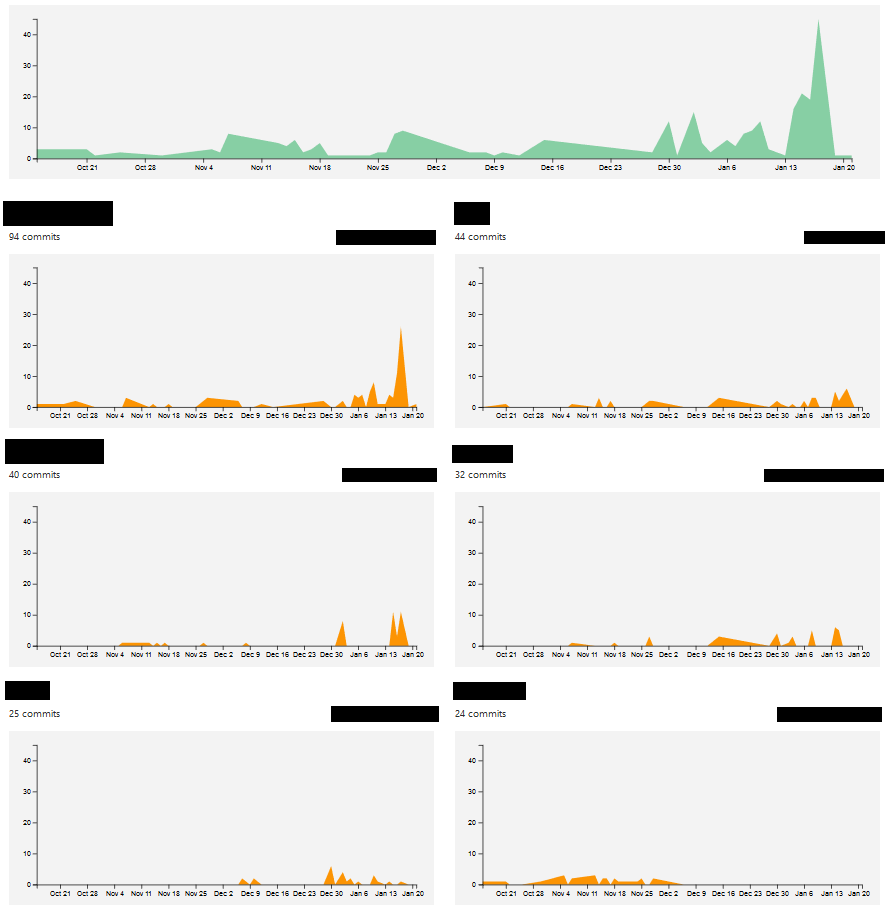
\includegraphics[scale=0.4]{slike/aktivnost.PNG} %veličina slike u odnosu na originalnu datoteku i pozicija slike
			\centering
			\caption{Primjer slike s potpisom}
			\label{fig:promjene}
		\end{figure}
		
		\begin{figure}[H]
			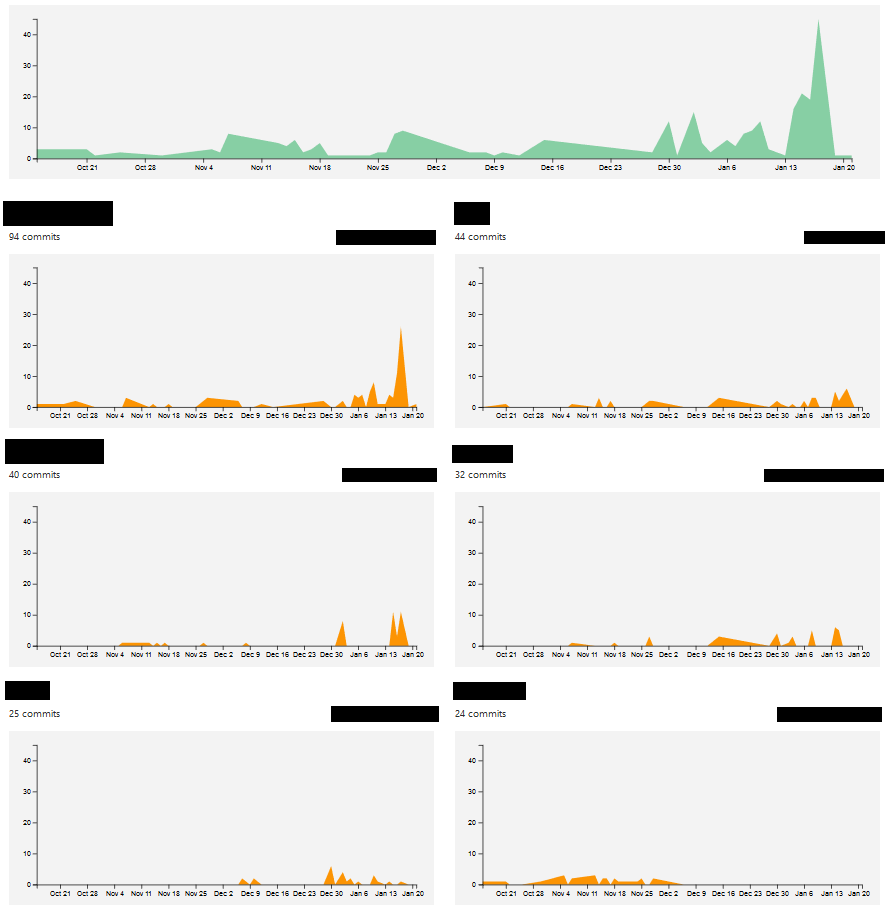
\includegraphics[width=\textwidth]{slike/aktivnost.PNG} %veličina u odnosu na širinu linije
			\caption{Primjer slike s potpisom 2}
			\label{fig:promjene2} %label mora biti drugaciji za svaku sliku
		\end{figure}
		
		Referenciranje slike \ref{fig:promjene2} u tekstu.
		
		\eject
		
	